% !TeX encoding = UTF-8
% !TeX spellcheck = en_GB
% !TeX root = ../ThesisTemplate_AndreGuerra.tex
%%%%%%%%%%%%%%%%%%% 10_Intro.tex %%%%%%%%%%%%%%%%%%%%%%%%%%%%%%%%%%
%
% PhD Thesis - Introduction
% André Guerra
%
% 12/Dec/2017
%
%%%%%%%%%%%%%%%%%%%%%%%%%%%%%%%%%%%%%%%%%%%%%%%%%%%%%%%%%%%%%%%%%%%


% ---------------------------------------------
% ---------------------------------------------
\chapter{Introduction}
\label{chp:Introduction}

This file is just a mockup to show the functionalities used on this template.

With this template I suggest to add numbers with units as \SI{30}{kg}.
This package also allows to add just units, \si{kg}, to write numbers in a compact format, \num{1e3}, and to even add that small space between orders of magnitude, \num{36000}.
This package is called \emph{siunitx}.

Figures are added as usual, but are referenced using \emph{hyperef} package.
This means that the code for~\autoref{fig:HumSat_Xatcobeo} can be seen below, but the reference is done with the command \emph{\textbackslash{}autoref}.
This reference system also works for the document structure, i.e. it is possible to reference~\autoref{chp:Introduction} or er even~\autoref{sec:Intro_Motivation}.
References to bibliography is done as usual, i.e. Ref.~\cite{Guerra2016}.
%
\begin{figure}[!htb]
    \centering
    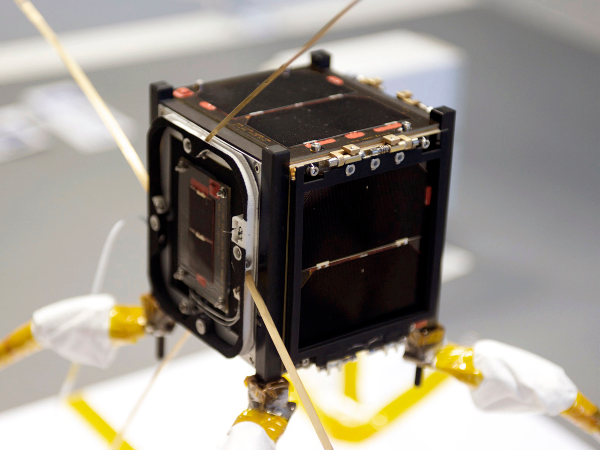
\includegraphics[width=0.5\textwidth]{Xatcobeo.pdf} %Xatcobeo.jpg
    \caption{Xatcobeo satellite photography (image from ESA-UVigo/INTA).}
    \label{fig:HumSat_Xatcobeo}
\end{figure}

Furthermore, there is a package to allow multiple figures to be defined within the same main figure, \emph{subcaption}.
With the code below, the author has the possibility to reference both the main figure (\autoref{fig:Trials_Setup}), or to reference each individual one (\autoref{fig:Trials_Setup_NetworkA} and \autoref{fig:Trials_Setup_NetworkB}).
%
\begin{figure}[!htb]
    \centering
    \begin{subfigure}[b]{0.48\textwidth}
        \centering
        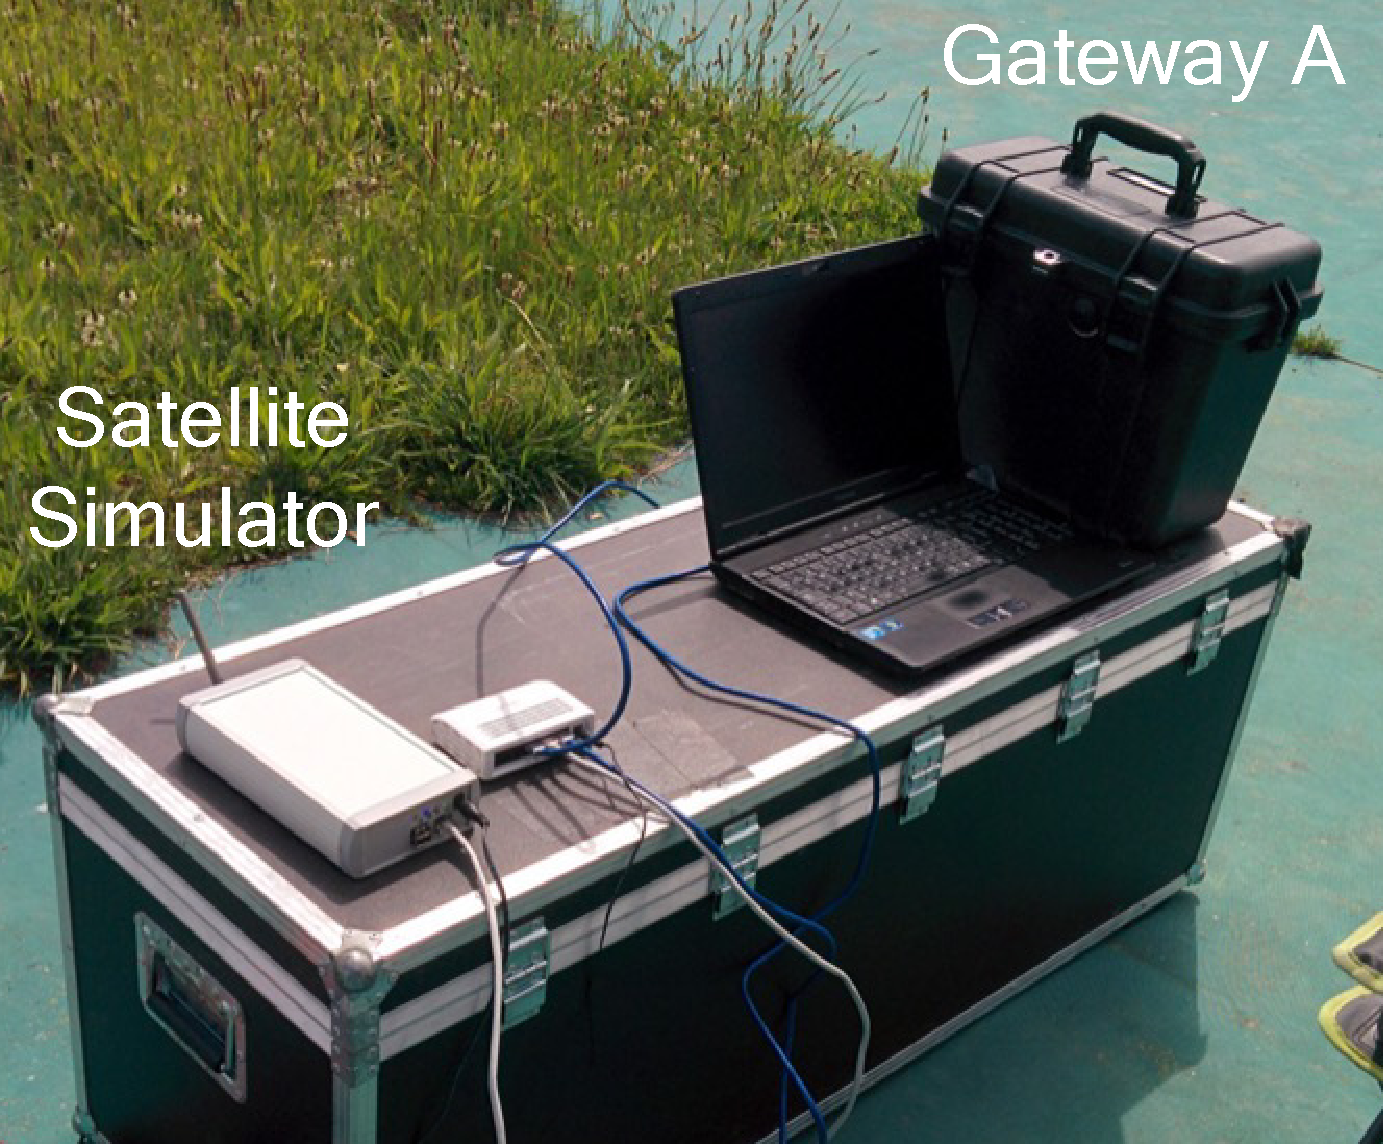
\includegraphics[width=0.97\textwidth]{NetworkA_FieldTry.pdf} %NetworkA_FieldTry.pdf
        \caption{Network A}
        \label{fig:Trials_Setup_NetworkA}
    \end{subfigure}
    \\ % To add a paragraph between figures.
    % Other options are possible, such as ~ or simply a blank line.
    \begin{subfigure}[b]{0.48\textwidth}
        \centering
        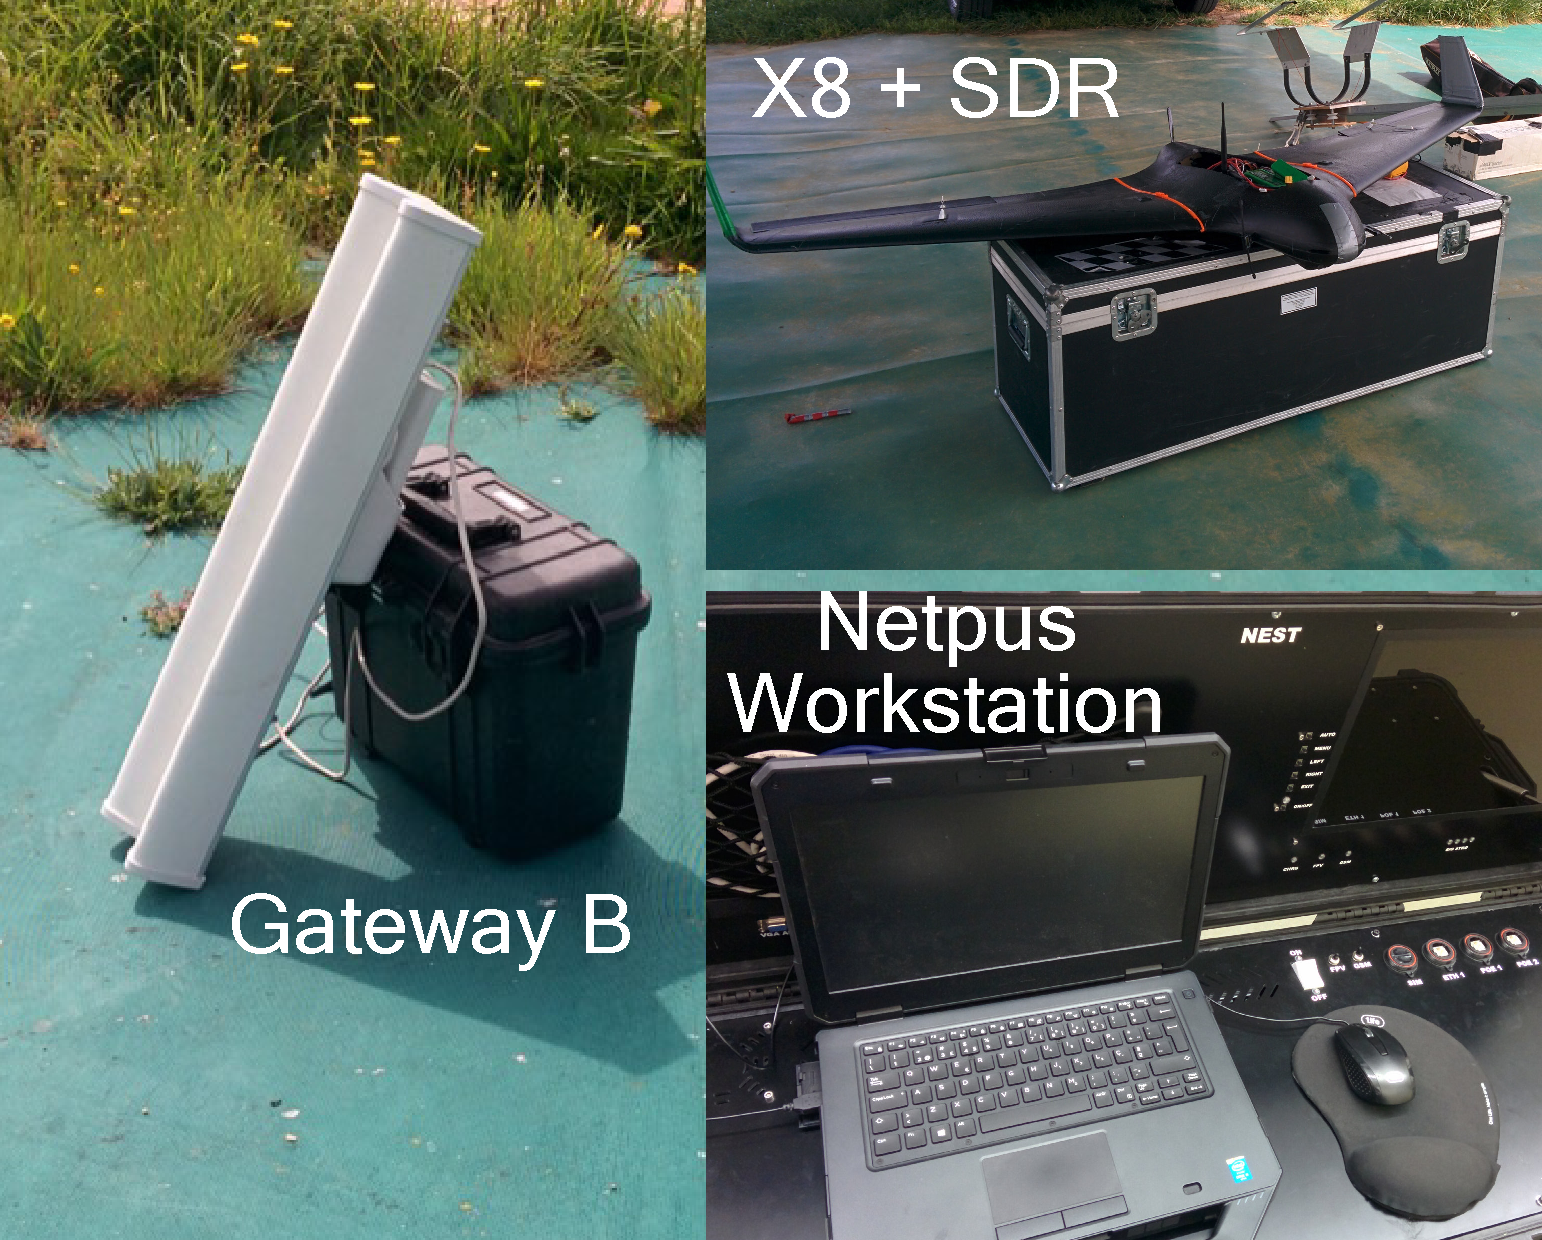
\includegraphics[width=1\textwidth]{NetworkB_FieldTry.pdf} %NetworkB_FieldTry.jpg
        \caption{Network B}
        \label{fig:Trials_Setup_NetworkB}
    \end{subfigure}
    \caption{Field trials operational setup.}
    \label{fig:Trials_Setup}
\end{figure}

For tables, besides the common \emph{booktabs} package, there is an extra one, \emph{threeparttable}, to create tables with footnotes in it.
The code for a table like this is shown below in~\autoref{tab:satcomm_comparison}
%
\begin{table}[!htb]
    %\scriptsize%\tiny
    \small
    %\setlength\tabcolsep{3.5pt}
    %\renewcommand{\arraystretch}{1.5}
    \centering
    \caption{Main characteristics of the satellite communication systems described (data from Refs.~\cite{Guerra2016}).}
    \label{tab:satcomm_comparison}
    \begin{threeparttable}
        \begin{tabular}{c >{\centering}m{1.8cm} c >{\centering}m{1.8cm} >{\centering}m{1.5cm} >{\centering}m{2cm} m{1.4cm}<{\centering}}
            \toprule
            System                      
            & Orbit Altitude [\si{km}]
            & Comm. Type    & Transmitting Power\tnote{\textdagger}\ \ [\si{W}]
            & Data rate\tnote{\textdagger}\ \ [\si{kbits/s}]   & Data Amount per Message\tnote{\textdagger}\ [\si{bytes}]
            & System of systems \\
            \midrule
            \multirow{2}[0]{*}{INMARSAT}
            & \multirow{2}[0]{\hsize}{\centering\num{35800} (GEO)}
            & Voice         & 100
            & 100                                           & --\tnote{$\ast$}
            & \multirow{2}[0]{*}{No} \\
            &
            & Data          & 9
            & --\tnote{$\ast$}                              & \num{6400}
            &  \\
            \multirow{2}[0]{*}{Iridium} 
            & \multirow{2}[0]{\hsize}{\centering780 (LEO)}
            & Voice         & 31
            & 134                                           & -
            & \multirow{2}[0]{*}{No} \\
            &
            & Data          & 1
            & 2.4                                           & 50
            &  \\
            Argos 
            & 800 (LEO)
            & Data          & 1
            & 4.8                                           & 31
            & No \\
            HumSat 
            & 600 (LEO)
            & Data          & 1
            & 1.2                                           & 32
            & Yes \\
            \bottomrule
        \end{tabular}
        \begin{tablenotes}
            \item[\textdagger] Values shown are top limits.
            \item[$\ast$] Information not available.
        \end{tablenotes}
    \end{threeparttable}
\end{table}

There is a package loaded to prevent figures from overstepping sections, \emph{placeins}.
This package besides being active for section, can also be modified to work with subsection.
Nevertheless, if the problem with a float going to the next subsection is localised, the command \emph{\textbackslash{}FloatBarrier} can be used after the float to prevent it from moving past that point.

Apart from these writing aspects, a package to handle and print a nomenclature was added, \emph{nomencl}.
To work with this package the author should add definitions as can be seen in file \textbf{01\_FrontMatter/Thesis\_Nomenclature}.



% ---------------------------------------------
% !TeX encoding = UTF-8
% !TeX spellcheck = en_GB
% !TeX root = ../ThesisTemplate_AndreGuerra.tex
%%%%%%%%%%%%%%%%%%% 11_Intro_Motivation.tex %%%%%%%%%%%%%%%%%%%%%%%%%%%%%%%
%
% PhD Thesis - Introduction - Motivation
% André Guerra
%
% 13/Dec/2017
%
%%%%%%%%%%%%%%%%%%%%%%%%%%%%%%%%%%%%%%%%%%%%%%%%%%%%%%%%%%%%%%%%%%%


% ---------------------------------------------
% ---------------------------------------------
\section{Motivation for small satellite oceanography}
\label{sec:Intro_Motivation}

{\small\textit{\lipsum[1-2]}}

% ---------------------------------------------
\subsection{The case for small satellite SAR}

{\small\textit{\lipsum[1-2]}}


% end of file 11_Intro_Motivation.tex
%%%%%%%%%%%%%%%%%%%%%%%%%%%%%%%%%%%%%%%%%%%%%%%%%%%%%%%%%%%%%%%%%%%

% ---------------------------------------------
% !TeX encoding = UTF-8
% !TeX spellcheck = en_GB
% !TeX root = ../Thesis_AndreGuerra.tex
%%%%%%%%%%%%%%%%%%% 12_Intro_CoordinatedObeservation.tex %%%%%%%%%%%%%%%%%%%%%%%%%%%%%%%
%
% PhD Thesis - Introduction - Coordinated Observation
% André Guerra
%
% 13/Dec/2017
%
%%%%%%%%%%%%%%%%%%%%%%%%%%%%%%%%%%%%%%%%%%%%%%%%%%%%%%%%%%%%%%%%%%%


% ---------------------------------------------
% ---------------------------------------------
\section{Coordinated observation with autonomous platforms}
\label{sec:Intro_CoordinatedObeservation}

{\small\textit{\lipsum[1-2]}}

% ---------------------------------------------
\subsection{Communication network}
\label{sec:Intro_CommNetwork}

{\small\textit{\lipsum[1-2]}}

% ---------------------------------------------
\subsection{The Portuguese case}
\label{sec:Intro_Portugal}

{\small\textit{\lipsum[1-2]}}


% end of file 12_Intro_CoordinatedObeservation.tex
%%%%%%%%%%%%%%%%%%%%%%%%%%%%%%%%%%%%%%%%%%%%%%%%%%%%%%%%%%%%%%%%%%%

% ---------------------------------------------
% !TeX encoding = UTF-8
% !TeX spellcheck = en_GB
% !TeX root = ../ThesisTemplate_AndreGuerra.tex
%%%%%%%%%%%%%%%%%%% 13_Intro_ThermalAnalysis.tex %%%%%%%%%%%%%%%%%%
%
% PhD Thesis - Introduction - Thermal Analysis
% André Guerra
%
% 18/Dec/2017
%
%%%%%%%%%%%%%%%%%%%%%%%%%%%%%%%%%%%%%%%%%%%%%%%%%%%%%%%%%%%%%%%%%%%


% ---------------------------------------------
% ---------------------------------------------
\section{Spacecraft design -- Thermal analysis and ensued accelerations}
\label{sec:Intro_Thermal}

{\small\textit{\lipsum[1-2]}}

% ---------------------------------------------
\subsection{Thermal radiation implications}
\label{sec:Intro_ThermalImplications}

{\small\textit{\lipsum[1-2]}}


% end of file 13_Intro_ThermalAnalysis.tex
%%%%%%%%%%%%%%%%%%%%%%%%%%%%%%%%%%%%%%%%%%%%%%%%%%%%%%%%%%%%%%%%%%%

% ---------------------------------------------
% ---------------------------------------------
\section{Objectives and outline}
\label{sec:Intro_OutlineObjectives}



% end of file 10_Intro.tex
%%%%%%%%%%%%%%%%%%%%%%%%%%%%%%%%%%%%%%%%%%%%%%%%%%%%%%%%%%%%%%%%%%%